\documentclass[a4paper]{report}
% Some basic packages
\usepackage[utf8]{inputenc}
\usepackage[T1]{fontenc}
\usepackage{textcomp}
\usepackage[english]{babel}
\usepackage{url}
\usepackage{graphicx}
\usepackage{float}
\usepackage{booktabs}
\usepackage{enumitem}

\pdfminorversion=7

% Don't indent paragraphs, leave some space between them
\usepackage{parskip}

% Hide page number when page is empty
\usepackage{emptypage}
\usepackage{subcaption}
\usepackage{multicol}
\usepackage{xcolor}

% Other font I sometimes use.
% \usepackage{cmbright}

% Math stuff
\usepackage{amsmath, amsfonts, mathtools, amsthm, amssymb}
% Fancy script capitals
\usepackage{mathrsfs}
\usepackage{cancel}
% Bold math
\usepackage{bm}
% Some shortcuts
\newcommand\N{\ensuremath{\mathbb{N}}}
\newcommand\R{\ensuremath{\mathbb{R}}}
\newcommand\Z{\ensuremath{\mathbb{Z}}}
\renewcommand\O{\ensuremath{\emptyset}}
\newcommand\Q{\ensuremath{\mathbb{Q}}}
\newcommand\C{\ensuremath{\mathbb{C}}}
\renewcommand\L{\ensuremath{\mathcal{L}}}

% Package for Petri Net drawing
\usepackage[version=0.96]{pgf}
\usepackage{tikz}
\usetikzlibrary{arrows,shapes,automata,petri}
\usepackage{tikzit}
\input{petri_nets_style.tikzstyles}

% Easily typeset systems of equations (French package)
\usepackage{systeme}

% Put x \to \infty below \lim
\let\svlim\lim\def\lim{\svlim\limits}

%Make implies and impliedby shorter
\let\implies\Rightarrow
\let\impliedby\Leftarrow
\let\iff\Leftrightarrow
\let\epsilon\varepsilon

% Add \contra symbol to denote contradiction
\usepackage{stmaryrd} % for \lightning
\newcommand\contra{\scalebox{1.5}{$\lightning$}}

% \let\phi\varphi

% Command for short corrections
% Usage: 1+1=\correct{3}{2}

\definecolor{correct}{HTML}{009900}
\newcommand\correct[2]{\ensuremath{\:}{\color{red}{#1}}\ensuremath{\to }{\color{correct}{#2}}\ensuremath{\:}}
\newcommand\green[1]{{\color{correct}{#1}}}

% horizontal rule
\newcommand\hr{
    \noindent\rule[0.5ex]{\linewidth}{0.5pt}
}

% hide parts
\newcommand\hide[1]{}

% si unitx
\usepackage{siunitx}
\sisetup{locale = FR}

% Environments
\makeatother
% For box around Definition, Theorem, \ldots
\usepackage{mdframed}
\mdfsetup{skipabove=1em,skipbelow=0em}
\theoremstyle{definition}
\newmdtheoremenv[nobreak=true]{definitie}{Definitie}
\newmdtheoremenv[nobreak=true]{eigenschap}{Eigenschap}
\newmdtheoremenv[nobreak=true]{gevolg}{Gevolg}
\newmdtheoremenv[nobreak=true]{lemma}{Lemma}
\newmdtheoremenv[nobreak=true]{propositie}{Propositie}
\newmdtheoremenv[nobreak=true]{stelling}{Stelling}
\newmdtheoremenv[nobreak=true]{wet}{Wet}
\newmdtheoremenv[nobreak=true]{postulaat}{Postulaat}
\newmdtheoremenv{conclusie}{Conclusie}
\newmdtheoremenv{toemaatje}{Toemaatje}
\newmdtheoremenv{vermoeden}{Vermoeden}
\newtheorem*{herhaling}{Herhaling}
\newtheorem*{intermezzo}{Intermezzo}
\newtheorem*{notatie}{Notatie}
\newtheorem*{observatie}{Observatie}
\newtheorem*{exe}{Exercise}
\newtheorem*{opmerking}{Opmerking}
\newtheorem*{praktisch}{Praktisch}
\newtheorem*{probleem}{Probleem}
\newtheorem*{terminologie}{Terminologie}
\newtheorem*{toepassing}{Toepassing}
\newtheorem*{uovt}{UOVT}
\newtheorem*{vb}{Voorbeeld}
\newtheorem*{vraag}{Vraag}

\newmdtheoremenv[nobreak=true]{definition}{Definition}
\newtheorem*{eg}{Example}
\newtheorem*{notation}{Notation}
\newtheorem*{previouslyseen}{As previously seen}
\newtheorem*{remark}{Remark}
\newtheorem*{note}{Note}
\newtheorem*{problem}{Problem}
\newtheorem*{observe}{Observe}
\newtheorem*{property}{Property}
\newtheorem*{intuition}{Intuition}
\newmdtheoremenv[nobreak=true]{prop}{Proposition}
\newmdtheoremenv[nobreak=true]{theorem}{Theorem}
\newmdtheoremenv[nobreak=true]{corollary}{Corollary}

% End example and intermezzo environments with a small diamond (just like proof
% environments end with a small square)
\usepackage{etoolbox}
\AtEndEnvironment{vb}{\null\hfill$\diamond$}%
\AtEndEnvironment{intermezzo}{\null\hfill$\diamond$}%
% \AtEndEnvironment{opmerking}{\null\hfill$\diamond$}%

% Fix some spacing
% http://tex.stackexchange.com/questions/22119/how-can-i-change-the-spacing-before-theorems-with-amsthm
\makeatletter
\def\thm@space@setup{%
  \thm@preskip=\parskip \thm@postskip=0pt
}


% Exercise 
% Usage:
% \exercise{5}
% \subexercise{1}
% \subexercise{2}
% \subexercise{3}
% gives
% Exercise 5
%   Exercise 5.1
%   Exercise 5.2
%   Exercise 5.3
\newcommand{\exercise}[1]{%
    \def\@exercise{#1}%
    \subsection*{Exercise #1}
}

\newcommand{\subexercise}[1]{%
    \subsubsection*{Exercise \@exercise.#1}
}


% \lecture starts a new lecture (les in dutch)
%
% Usage:
% \lecture{1}{di 12 feb 2019 16:00}{Inleiding}
%
% This adds a section heading with the number / title of the lecture and a
% margin paragraph with the date.

% I use \dateparts here to hide the year (2019). This way, I can easily parse
% the date of each lecture unambiguously while still having a human-friendly
% short format printed to the pdf.

\usepackage{xifthen}
\def\testdateparts#1{\dateparts#1\relax}
\def\dateparts#1 #2 #3 #4 #5\relax{
    \marginpar{\small\textsf{\mbox{#1 #2 #3 #5}}}
}

\def\@lecture{}%
\newcommand{\lecture}[3]{
    \ifthenelse{\isempty{#3}}{%
        \def\@lecture{Lecture #1}%
    }{%
        \def\@lecture{Lecture #1: #3}%
    }%
    \subsection*{\@lecture}
    \marginpar{\small\textsf{\mbox{#2}}}
}



% These are the fancy headers
\usepackage{fancyhdr}
\pagestyle{fancy}

% LE: left even
% RO: right odd
% CE, CO: center even, center odd
% My name for when I print my lecture notes to use for an open book exam.
% \fancyhead[LE,RO]{Gilles Castel}

\fancyhead[RO,LE]{\@lecture} % Right odd,  Left even
\fancyhead[RE,LO]{}          % Right even, Left odd

\fancyfoot[RO,LE]{\thepage}  % Right odd,  Left even
\fancyfoot[RE,LO]{}          % Right even, Left odd
\fancyfoot[C]{\leftmark}     % Center

\makeatother




% Todonotes and inline notes in fancy boxes
\usepackage{todonotes}
\usepackage{tcolorbox}

% Make boxes breakable
\tcbuselibrary{breakable}

% Verbetering is correction in Dutch
% Usage: 
% \begin{verbetering}
%     Lorem ipsum dolor sit amet, consetetur sadipscing elitr, sed diam nonumy eirmod
%     tempor invidunt ut labore et dolore magna aliquyam erat, sed diam voluptua. At
%     vero eos et accusam et justo duo dolores et ea rebum. Stet clita kasd gubergren,
%     no sea takimata sanctus est Lorem ipsum dolor sit amet.
% \end{verbetering}
\newenvironment{verbetering}{\begin{tcolorbox}[
    arc=0mm,
    colback=white,
    colframe=green!60!black,
    title=Opmerking,
    fonttitle=\sffamily,
    breakable
]}{\end{tcolorbox}}

% Noot is note in Dutch. Same as 'verbetering' but color of box is different
\newenvironment{noot}[1]{\begin{tcolorbox}[
    arc=0mm,
    colback=white,
    colframe=white!60!black,
    title=#1,
    fonttitle=\sffamily,
    breakable
]}{\end{tcolorbox}}




% Figure support as explained in my blog post.
\usepackage{import}
\usepackage{xifthen}
\usepackage{pdfpages}
\usepackage{transparent}
\newcommand{\incfig}[1]{%
    \def\svgwidth{\columnwidth}
    \import{./figures/}{#1.pdf_tex}
}

% Fix some stuff
% %http://tex.stackexchange.com/questions/76273/multiple-pdfs-with-page-group-included-in-a-single-page-warning
\pdfsuppresswarningpagegroup=1


% My name
\author{Bruno M. Pacheco}

 
\begin{document}
 
\title{Exercícios de Busca}
\author{Bruno M. Pacheco (16100865)\\
DAS5341 - Inteligência Artificial Aplicada a Controle e Automação}
 
\maketitle
 
\exercise{3}

\subexercise{a}

Um estado precisa representar a quantidade de missionários e canibais em uma das margens (uma vez que a outra margem terá um valor complementar) e em qual margem se encontra o barco.

Podemos representar os estados através do conjunto $E = \N\times \N\times \{0,1\} $, de forma que um estado $e\in E$ seja da forma $e = \left( m, c, b \right) $, onde $m$ indica a quantidade de missionários na margem inicial do rio, $c$ a quantidade de canibais nessa mesma margem, e $b$ caso o barco esteja na margem original (1) ou não.

\subexercise{b}

O estado inicial pode ser representado por \[
e_i = \left( 3,3,1 \right) 
,\] enquanto o final pode ser \[
e_f = \left( 0,0,0 \right) 
.\] 

\subexercise{c}

Podemos descrever as operações através de funções $f_1,f_2,f_3,f_4,f_5,g_1,g_2,g_3,g_4,g_5: E \longrightarrow E$ de forma que 
\begin{align*}
    f_1: E &\longrightarrow E \\
    \left( m,c,1 \right)  &\longmapsto f_1(\left( m,c,1 \right) ) = \left( m-1,c,0 \right) 
,\end{align*}
\begin{align*}
    f_2: E &\longrightarrow E \\
    \left( m,c,1 \right)  &\longmapsto f_1(\left( m,c,1 \right) ) = \left( m-2,c,0 \right) 
,\end{align*}
\begin{align*}
    f_3: E &\longrightarrow E \\
    \left( m,c,1 \right)  &\longmapsto f_1(\left( m,c,1 \right) ) = \left( m,c-1,0 \right) 
,\end{align*}
\begin{align*}
    f_4: E &\longrightarrow E \\
    \left( m,c,1 \right)  &\longmapsto f_1(\left( m,c,1 \right) ) = \left( m,c-2,0 \right) 
\end{align*}
e
\begin{align*}
    f_5: E &\longrightarrow E \\
    \left( m,c,1 \right)  &\longmapsto f_1(\left( m,c,1 \right) ) = \left( m-1,c-1,0 \right) 
\end{align*}
sejam as operações de travessia no sentido da margem desejada, ou seja, possuem como pré-requisito que $b=1$ e que tenham suficientes passageiros para a mesma na margem de origem. De forma equivalente, as operações $g_i=f_i^{-1}, i=1,\ldots,5$ fazem o mesmo mas no sentido oposto, com pré-requisitos, portanto, exatamente opostos.

\subexercise{d}

\begin{figure}[H]
    \centering
    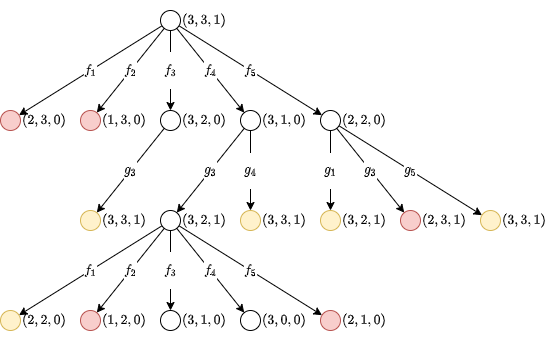
\includegraphics[width=0.8\textwidth]{figures/lista1_3_d.png}
\end{figure}

Os estados já visitados foram marcados em amarelo enquanto os estados proibidos foram marcados em vermelho.

\subexercise{e}

Considerando o pior caso (desconsiderando podas e transições impossíveis), cada nó se ramifica em outros 5 nós uma vez que são 5 possíveis transições para o barco em cada lado da margem. Além disso, pode-se estimar que a solução utiliza até duas transições para atravessar cada pessoa. Dessa forma, estimamos o tamanho em \[
1 + 5 + 5^2 + \ldots + 5^{12} = 240\text{M nós}
\] no pior caso.

\subexercise{f}

Como é um problema simples com uma poda agressiva (elimina muitos estados), estimo pouca diferença na eficiência dos métodos. Como é de interesse para o problema encontrar uma solução eficiente, acredito que a busca em largura seria mais efetiva.

\exercise{5}

\subexercise{a}

Podemos modelar os estados como uma matriz $n\times n$ normal (pela definição do enunciado) e um valor binário que indica se a matriz é um quadrado mágico ou não.

Dessa forma, podemos escrever o conjunto de estados \[
E = \left\{ \left( M, m \right) \in  \Z_{n\times n} \times \{0,1\} : M\text{ é normal} \right\} 
.\] 

\subexercise{b}

O estado inicial $e_i=\left( M_i, b_i \right) $ pode ser composto por matriz normal $M_i$ e valor $b_i$, enquanto o final $e_f=\left( M_f,b_f \right) $ é qualquer estado com $b_f=1$.

\subexercise{c}

As operações possíveis são trocas de valores entre os campos da matriz, mantendo-a normal. Nota-se também que o valor de $b$ deve ser corrigido a cada operação para condizer com a matriz resultante.

\subexercise{d}

Para que o desenho se tornasse factível, somente alguns nós de uma árvore para uma matriz $3\times 3$ foi desenhada.

\begin{figure}[H]
    \centering
    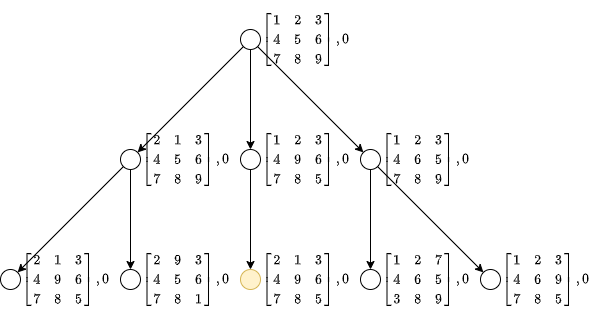
\includegraphics[width=0.8\textwidth]{figures/lista1_5_d.png}
\end{figure}

\subexercise{e}

Uma árvore extremamente eficiente teria somente todas as permutações possíveis dos elementos da matriz, ou seja, para uma matriz $3\times 3$, seriam \[
9! = 362880\text{ nós}
.\] 

\subexercise{f}

Como a árvore é bastante grande e as soluções dificilmente são "rasas", o algoritmo de busca em largura poderia acabar sendo penoso por seu custo de memória. Dessa forma, eu optaria pelo algoritmo de busca em profundidade. Além disso, devem haver muitos estados metas ao longo da árvore, uma vez que as transições são permutáveis, o que favorece a busca em profundidade.

\exercise{6}

\subexercise{a}

Precisamos representar a posição de cada caixa em cada pilha. Para isso, podemos utilizar uma linguagem $L\subseteq \Sigma^*$ sobre o alfabeto $\Sigma=\{a,b,c,d,e,f,g\} $. Para garantir que as palavras dessa linguagem representam algum empilhamento das caixa, definimos \[
L = \left\{ w\in \Sigma^* : \|w\| = \|Alph\left( w \right) \|\right\} 
,\] ou seja, a quantidade de letras no alfabeto de cada palavra deve ser idêntica ao tamanho da palavra, evitando palavras com letras repetidas.

Assim, podemos definir os estados como \[
E = \left\{ \left( p_1,p_2,p_3 \right) \in L\times L\times L : \|p_1\|+\|p_2\|+\|p_3\| = \|\Sigma\| \right\} 
.\] Note que a condição sobre os estados junto com a restrição sobre as palavras resulta na ausência de uma mesma caixa em múltiplas pilhas ($p_1,p_2,p_3$).

\subexercise{b}

\[
e_i = \left( abc, de, fg \right) 
\] e \[
e_f = \left( \epsilon, abcgf, ed \right) 
.\] 

\subexercise{c}

A movimentação das caixas pode ser modelada pelas funções $f_{i,j}: E \longrightarrow E$ que movimentam uma caixa da pilha $i$ para a pilha $j$, de forma que, por exemplo,
\begin{align*}
    f_{1,2}: E &\longrightarrow E \\
    \left( p_1,p_2,p_3 \right)  &\longmapsto f_{1,2}(\left( p_1,p_2,p_3 \right) ) = \left( p_1 \setminus last\left( p_1 \right), p_2\cdot last\left( p_1 \right)  , p_3 \right) 
,\end{align*}
onde $last(\cdot )$ indica a última letra de uma palavra e as demais operações indicam remoção e concatenação.

\subexercise{d}

Considerou-se somente um ramo da árvore para fins práticos.

\begin{figure}[H]
    \centering
    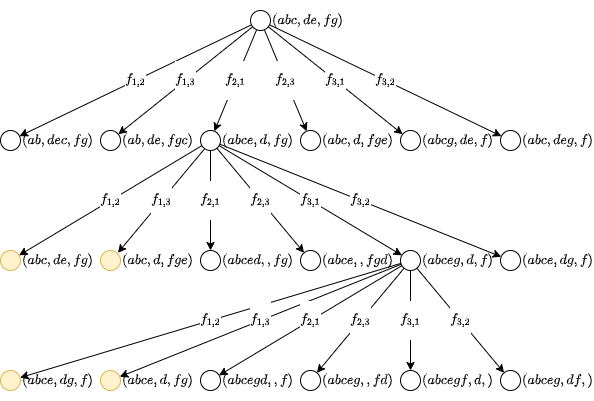
\includegraphics[width=0.8\textwidth]{figures/lista1_6_d.png}
\end{figure}

\subexercise{e}

Considerando o pior caso (desconsiderando podas e transições impossíveis), cada nó se ramifica em 6 outros, enquanto a solução encontra-se a 13 transições. Dessa forma, a árvore possuirá \[
    1 + 6 + \ldots + 6^13 = 15.672.832.819\text{ nós}
.\] 

\subexercise{f}

Com essa quantidade de nós, o uso de memória se torna um limitante, logo, a busca em largura pode se tornar impraticável. Além disso, pela permutabilidade das transições, a árvore deve ser bem povoada por estados metas, ou seja, a busca em profundidade não será muito ineficiente.

\end{document}
